\chapter{Uživatelský manuál programu Sound Analyzer}


\section{Slovníček pojmů užitých v této kapitole}

\subsection{Frequency indexes}

Indexy kmitočtů které budou počítány. Jsou to čísla $n$ ze vzorce \ref{vztah:DFT}.


\subsection{Sampling frequency}

Vzorkovací kmitočet.

\subsection{Scale}

Měřítko specifikuje zobrazený rozsah grafů a je znázorněno na pravítkách.

\subsection{Segment length}
\label{sec:segmentlegth}

Segmentem je myšlen vektor určité délky, reprezentující část signálu. Komponenta \emph{Recorder} čte ze vstupu (nebo přehrává) právě po úsecích této délky.

\subsection{Segment overlap}
\label{sec:segmentoverlap}

Komponenta \emph{Goertzel} umí pracovat s větší délkou segmentu než s tou, kterou načte ze vstupu. \emph{Segment overlap} je délka z předchozích vzorků, o kterou se rozšíří segment (vstupní vektor).


\section{Okno aplikace}

Na obrázku \ref{obr:manual1} vidíme základní obrazovku programu \emph{Sound Analyzer}.
Pravítka slouží k odečítání časů a velikostí amplitud jednoho nebo dvou grafů. Spodní lišta slouží k přepínání pohledů na signál. Konečně navigační pole slouží ke konfiguraci a zobrazuje důležité statistické informace o signálu. 

\begin{figure}
  \begin{center}
    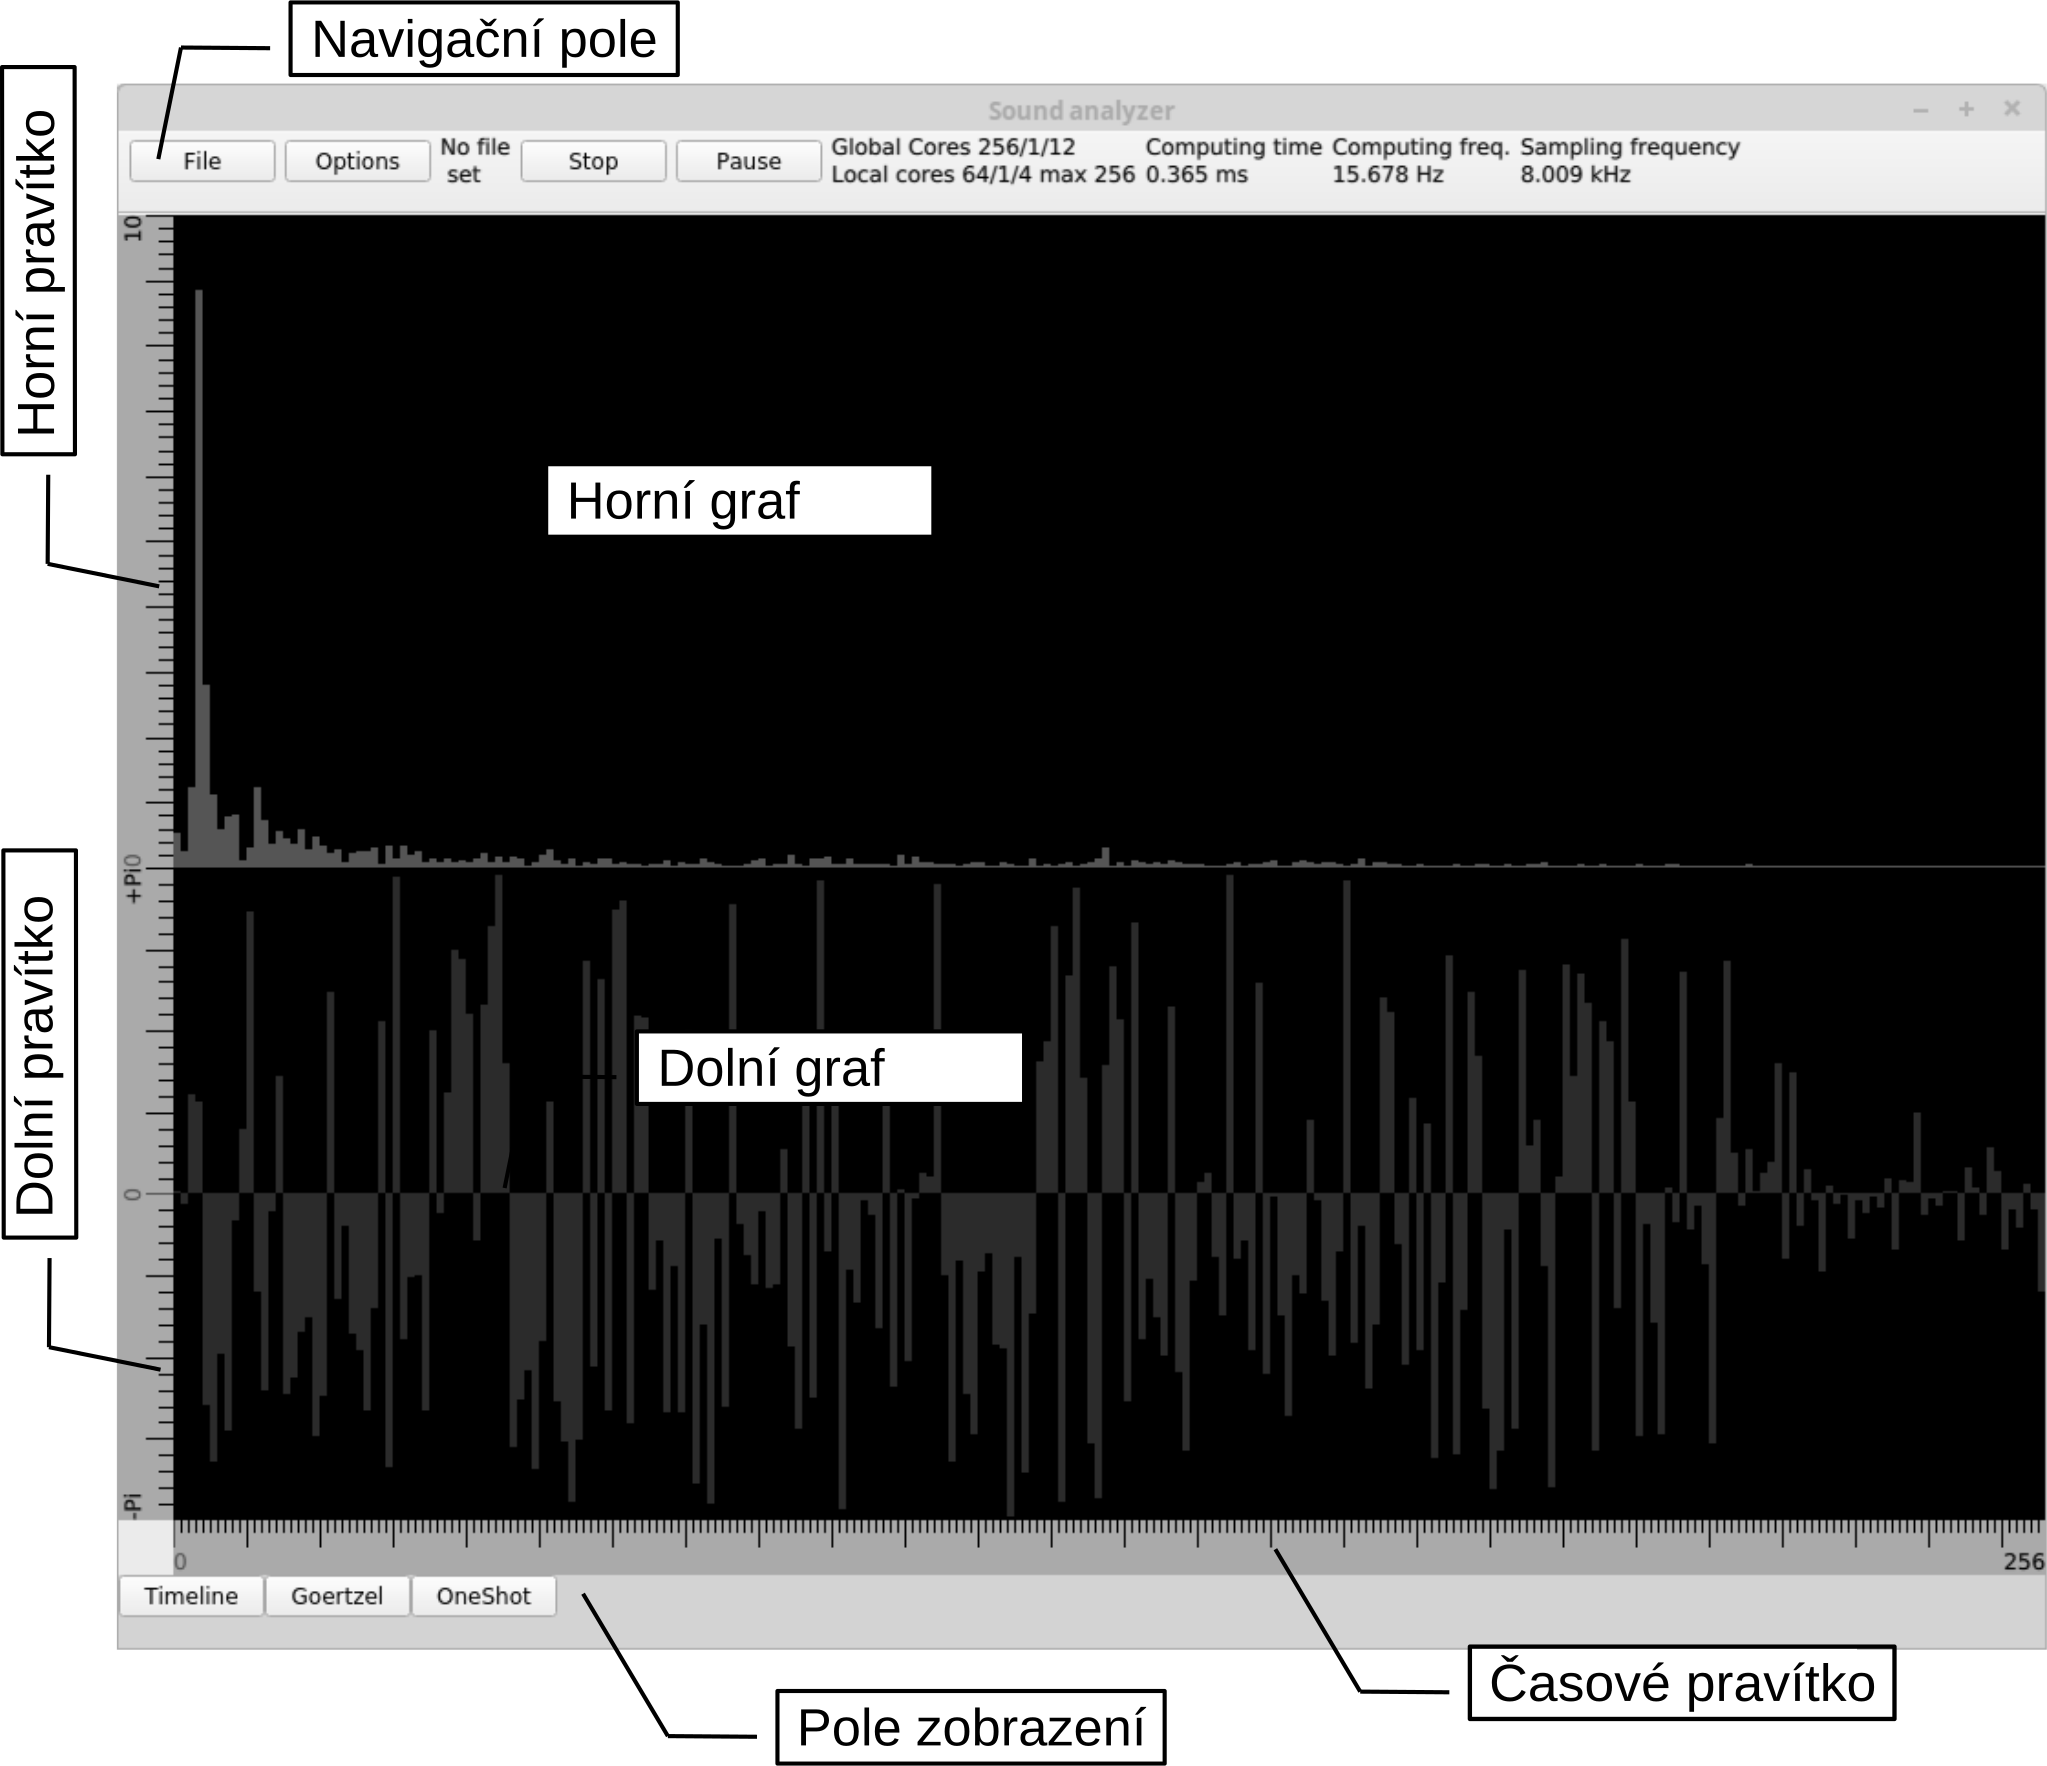
\includegraphics[scale=.65]{obr/manual1}
  \end{center}
  \caption{Pohled na aplikaci Sound Analyzer}
  \label{obr:manual1}
\end{figure}

\section{Horní graf}
\label{sec:topgraph}

Horní graf má dva režimy zobrazení. V zobrazení typu \emph{Goertzel} a \emph{OneShot} reprezentuje amplitudu. V režimu zobrazení \emph{Timeline} zobrazuje průběh signálu levého kanálu.
Ten se neposouvá, jinak řečeno, vždy když se načte segment, je zobrazen místo segmentu předcházejícího. Pokud je rychlost změn větší než obnovovací rychlost GUI knihovny \emph{Qt} zobrazený segment je zahozen a zobrazuje se ten poslední.

Zobrazení \emph{Timeline} může být dvougrafové(stereo) nebo grafem přes celou velikost okna(Mono). To je možno nastavit přepínačem \emph{Channels} a kartě \emph{Recorder} z dialogu \emph{Options}.


Měřítko v horizontálním směru je popsané v sekci časové pravítko \ref{sec:timeruler}.


Měřítko ve vertikálním směru je popsané v sekci Dolní a horní pravítko \ref{sec:vertruler}.


\section{Dolní graf}


I dolní graf má dva režimy zobrazení. V zobrazení typu \emph{Goertzel} a \emph{OneShot} reprezentuje fázi. V režimu zobrazení \emph{Timeline} zobrazuje průběh signálu pravého kanálu. Ten se cyklicky překresluje, jak je blíže popsáno o horního grafu \ref{sec:topgraph}.

Měřítka, stejně jako u grafu horního jsou popsány v sekcích o pravítkách  \ref{sec:timeruler}, \ref{sec:vertruler}.

\section{Horní a dolní pravítko}
\label{sec:vertruler}

V zobrazení typu \emph{Goertzel} a \emph{OneShot} reprezentuje amplitudu v rozsahu od $0$ do $y_{max}$. V režimu zobrazení \emph{Timeline} zobrazuje průběh signálu v rozsahu $-y_{max}$,$y_{max}$. Rozsah $y_{max}$ lze měnit jednak klávesovými zkratkami, jednak rozbalovacím seznamem \emph{Scale} na kartě \emph{General} z dialogu \emph{Options}.

\section{Časové pravítko}
\label{sec:timeruler}

V režimu \emph{Timeline} je na vodorovné ose vynesen počet vzorků které jsou najednou načteny ze vstupu. Je to současně nastavená hodnota \emph{Segment length} na kartě \emph{Recorder} v dialogu \emph{Options}. V režimu \emph{Goertzel} je na této ose počet počítaných harmonických, uvedených v seznamu \emph{Frequency indexes} na kartě \emph{Goertzel} v dialogu \emph{Options}. V režimu \emph{OneShot} se počítají všechny možné kmitočty signálu popsaném v souboru z \emph{Matlabu}. Na vodorovné ose je tedy počet kmitočtů, číselně roven délce zkoumaného signálu.

\section{Pole zobrazení}

V \emph{poli zobrazení} jsou tři tlačítka reprezentující tři režimy. Jsou to jediné akce, které můžete provádět za běhu.


Kromě změny zobrazení, tyto tlačítka přestavují toky dat mezi komponentami, jak je patrno z obrázku \ref{sec:sablockscheme}. Proto se při přepnutí z jednoho režimu do druhého a~zpět zobrazí implicitní sinus. Při přepnutí fronty se totiž segment se zobrazovanými daty musí vrátit.

\subsection{Timeline}

Režim \emph{Timeline} zobrazuje syrová data ze vstupu tak jak jdou za sebou. Jeden graf zobrazuje jeden segment. Zobrazení se s přibývajícím čase neposouvá, ale jen se překreslí aktuální segment.

Pokud je frekvence příchozích segmentů vyšší než je zobrazovací frekvence knihovny \emph{Qt}, tak se segmenty jednoduše zahodí (a vidět je ten poslední).

\subsection{Goertzel}

Režim \emph{Goertzel} zobrazuje spektrum signálu, respektive jen jeho požadované harmonické. Na horizontální ose najdeme počet počítaných harmonických.

\subsection{OneShot}

Režim \emph{OneShot} je kompletní spektrum signálu dodaného ze souboru \emph{matlabu}.
Pokud je v tomto souboru více vektorů se signály, zobrazen se jen ten poslední.

\section{Navigační pole}

Zde uvedu informační a ovládací prvky navigačního pole zleva doprava.

\subsection{Tlačítko File}

\subsubsection{Open for reading}

Klasickým \emph{File dialogem} si můžeme vybrat \emph{wav} soubor, který bude přehráván po stisknutí tlačítka \emph{Start}. Protože přehráváním se současně udává takt, bude program i nadále fungovat v reálném čase. Je možné mít otevřený soubor buď jen pro čtení nebo jen pro zápis, nikoli oba současně.

\subsubsection{Open for writing}

Klasickým \emph{File dialogem} si můžeme vybrat \emph{wav} soubor, do kterého budou ukládány načtené vzorky ze vstupu. V případě že výstupní zařízení není schopno ukládat požadované množství dat, bude výstupní soubor poškozený. 

\subsubsection{Close file}

Tímto zrušíte obě předchozí volby. Nyní se bude počítat spektrum jen ze vstupu.

\subsubsection{Process mat file}

Tato funkce je v programu \emph{Sound Analyzer} nejen pro ladící účely. Provede spočtení všech harmonických signálu dodaného v souboru typu \emph{mat} vytvořeném v prostředí \emph{matlab}.

Soubor typu \emph{mat} může obsahovat více vektorů. V takovém případě se provede výpočet spektra všech vektorů, ale vidět v pohledu \emph{OneShot} je pouze poslední.

Výstupní soubor je pojmenovaný jako $<vstupní soubor>\_ap$. V tomto souboru jsou dvě,
respektive dvakrát více vektorů než v souboru vstupním (amplituda a fáze). Jméno vektoru s amplitudami
 je $<vstupní vektor>\_am$ a vektory s fázemi mají jména $<vstupní vektor>\_ph$.

\subsubsection{Quit}

Konec programu.

\subsection{Tlačítko Options}

Spustí dialog nastavení. Více v sekci \emph{Dialog nastavení} \ref{sec:settingdialog}

\subsection{Jméno souboru pro zápis/čtení}

Zde je jméno souboru pro zápis/čtení a informace o tom, v jakém režimu souborové operace jsou (zápis/čtení/nic).

\subsection{Tlačítko Start}

Tlačítko \emph{Start} slouží ke startu jak skenování vstupu, tak počítání spektra.
Aby se počítalo spektrum, je nutné zobrazit režim \emph{Goertzel}, jinak načtená data nejdou přes Goertzelův algoritmus, ale pouze se zobrazují.

Teprve začátkem zaznamenávání nebo přehrávání se aplikují změny v dialogu nastavení.

Kliknutím se text na tlačítku změní na \emph{Stop}.

\subsection{Tlačítko Pause}

Tlačítko \emph{Pause-Continue} funguje i když zrovna není zapnuto skenování. To znamená že když je stav \emph{zapauzovaný} a následně kliknete na tlačítko \emph{Start}, skenování se zinicializuje, ale vlastní skenování nepoběží.

\subsection{Počet jader použitých při výpočtech}
\label{sec:nkernels}

V tomto okénku je sedm údajů: Globální $N/C/M$, lokální $N/C/M$ a maximální počet jader současně spustitelných.  $N$ je počet počítaných kmitočtů, $C$ je počet kanálů a konečně $M$ je počet mezisoučtů. Globální počet jader je tedy celkový požadavek na výpočet a jeho velikost je $N\times C\times M$. Tři souřadnice udávají počet jader se v terminologii  \emph{OpenCL} nazývají $NDrange$. Naproti tomu lokální $NDRange$ je skutečná počet jader použitých současně pro výpočet. Určitě tedy platí, že $globální NDRange \geq lokální NDRange$. Je tu ještě jedno omezení. Globální souřadnice $NDRange$ 
musí být celočíselný násobek lokální souřadnice $NDRange$.

\subsection{Průměrný čas výpočtu spektra}

Vlákno programu \emph{Sound Analyzer}, které v cyklu počítá některé harmonické složky, obsahuje jednoduchou počítací smyčku. Jedna její iterace trvá právě tento zobrazený čas.

\subsection{Průměrná frekvence výpočtu spektra}

Jedná se o frekvenci, se kterou se provádí výpočty. Měla by být někde okolo\\
 $f_{vz} / <délka segmentu>$.

\subsection{Průměrná vzorkovací frekvence}
\label{sec:avgsamplingfreq}

Je spočtená hodnota braná z komponenty \emph{recorder}. Měla by být podobná
nastavenému \emph{vzorkovacímu kmitočtu}.

\section{Klávesové zkratky}

\begin{tabular}{|c|l|}
\hline
+&Zvýšení rozsahu vertiálního měřítka\\
-&Snížení rozsahu vertikálního měřítka\\
S&Start, Stop\\
space&Pause, Continue\\
\hline 
\end{tabular}


\section{Dialog nastavení}
\label{sec:settingdialog}


\subsection{Karta General}

\subsubsection{Automatic hide}

Automatické schovávání je jen hříčka pro \uv{hezčí} zobrazení, bez okraje okna, \emph{navigačního pole} a \emph{pole zobrazení}.

\subsubsection{Scale}

\emph{Vertikální měřítko} grafu se aplikuje okamžitě. Je to jedna z mála výjimek v dialogu \emph{Nastavení}. Pro rychlejší manipulaci s měřítkem jsou v programu klávesové zkratky $+,-$.

\subsection{Karta Recorder}

\emph{Recorder} je komponenta zodpovědná za načítání vzorků ze zvukového zařízení, případně přehrávání zvukového souboru. V případě že je to povoleno, posílá ještě data k uložení do souboru.

\subsubsection{Bits per sample}

Knihovna \emph{OpenAL} nabízí jen dvě možnosti přesnosti každého vzorku, 8bitovou a~16bitovou. Oba jsou to celočíselné typy.

\subsubsection{Channels}

Program \emph{Sound Analyzer} podporuje jak mono, tak stereo záznam, tak i přehrávání i~výpočet spektrálních čar. Modrou barvou je značen levý kanál, červenou pak pravý.

\subsubsection{Device}

Zde jde nastavit jen zařízení \emph{OpenAL Soft}. Knihovna \emph{OpenAL} nikdy žádné jiné zařízení nenabídla.

\subsubsection{Capture device}

\emph{Zařízení pro záznam zvuku} jsou obvykle tři. Výchozí je vždy \uv{vnitřní zvukový systém}, což je vždy mikrofon. Další zařízení, které tam vždy najdeme, je \uv{monitor vnitřního zvukového systému}, což je standardní zvukový výstup. Když ale zkusíme tento vstup nahrávat, zjistíme, že je nějak poškozen. Protože výchozí vstupní zařízení zvuk nedeformuje, jsem názoru, že jde o ochranu proti kopírování. Tento vstup totiž není zatížen ani minimálním šumem. Jako poslední je obvykle vstup, \uv{monitor HDMI výstupu}. Ten je nějak zkreslen podobně jako vstup předchozí.

\subsubsection{Sampling frequency}

Tato vzorkovací frekvence je použita pro inicializaci \emph{recorderu}. Pokud se podíváme na kmitočet spočtený \ref{sec:avgsamplingfreq}, zjistíme že pro \emph{zařízení-monitory}, nejsou tyto kmitočty totožné. V tom je to zkreslení.

\subsubsection{Segment length}

Délka segmentu (vektor vstupního signálu) v počtu vzorků. Více o něm je v sekci \emph{segment length} ve slovníčku pojmů \ref{sec:segmentlegth}.

\subsection{Karta Goertzel}

Tato karta se týká výhradně výpočtu spektrálních čar a knihovny \emph{OpenCL}.

\subsubsection{Segment overlap}

Počet vzorků, o které se rozšíří načtený segment. Více je ve slovníčku \emph{segment overlap} \ref{sec:segmentoverlap}.

\subsubsection{Frequency indexes}

V tomto textovém poli je seznam indexů spektrálních čar počítaného spektra. Nic nebrání tomu počítat jen stejnosměrnou složku (index 0) nebo několik málo kmitočtů, které nejdou po sobě. Jednotlivé celočíselné indexy jsou odděleny \uv{;} a pro lepší přehlednost mohou obsahovat libovolný počet přechodů na nové řádky.

\subsubsection{Tlačítko Set All}

Snazšího vyplnění předcházejícího pole dosáhneme tlačítkem \emph{Set All}. To nahradí jakýkoli obsah pole \emph{frequency indexes} indexy $0$ až $(segment\_length + segment\_overlap)$.

\subsubsection{Přepínač Device}

Tímto říkáme knihovne \emph{OpenCL}, zda požadujeme provádět výpočty hlavním procesorem nebo grafickým čipem.

\section{Příklad použití}

Předpokládejme, že bude chtít počítat stejnosměrnou složky signálu a současně amplitudu na kmitočtu 1kHz. Vzorkovací kmitočet použiji 8kHz.

Délku segmentu si zvolím. Například délka 200 vzorků by se načítala 200/8000s = 25ms. To je tak maximální doba, při které může třeba řečový signál považovat za stacionární.

Nejnižší, základní kmitočet, který jsem takto schopen měřit je 8000/200 = 40Hz. Nás ale zajímají indexy 0 - stejnosměrná složka a 1000Hz = 25 $\times$ 40Hz. Druhý index je tedy 25.

Ve shodě s předchozím nastavíme v dialogu \emph{nastavení} toto:\\

\begin{tabular}{|l|l|}
\hline
Bits per sample&16bit\\
Channels&Mono\\
Device&OpenAl Soft\\
Capture device&Vnitřní zvukový systém analogové stereo\\
Sampling frequency&8000\\
Segment length&200\\
Segment overlap&0\\
Frequency indexes&0;25;\\
Device&GPU\\
\hline 
\end{tabular}



